% Options for packages loaded elsewhere
\PassOptionsToPackage{unicode}{hyperref}
\PassOptionsToPackage{hyphens}{url}
%
\documentclass[
]{article}
\title{A7\_Holmes\_Brooke}
\author{Brooke Holmes}
\date{07/03/2022}

\usepackage{amsmath,amssymb}
\usepackage{lmodern}
\usepackage{iftex}
\ifPDFTeX
  \usepackage[T1]{fontenc}
  \usepackage[utf8]{inputenc}
  \usepackage{textcomp} % provide euro and other symbols
\else % if luatex or xetex
  \usepackage{unicode-math}
  \defaultfontfeatures{Scale=MatchLowercase}
  \defaultfontfeatures[\rmfamily]{Ligatures=TeX,Scale=1}
\fi
% Use upquote if available, for straight quotes in verbatim environments
\IfFileExists{upquote.sty}{\usepackage{upquote}}{}
\IfFileExists{microtype.sty}{% use microtype if available
  \usepackage[]{microtype}
  \UseMicrotypeSet[protrusion]{basicmath} % disable protrusion for tt fonts
}{}
\makeatletter
\@ifundefined{KOMAClassName}{% if non-KOMA class
  \IfFileExists{parskip.sty}{%
    \usepackage{parskip}
  }{% else
    \setlength{\parindent}{0pt}
    \setlength{\parskip}{6pt plus 2pt minus 1pt}}
}{% if KOMA class
  \KOMAoptions{parskip=half}}
\makeatother
\usepackage{xcolor}
\IfFileExists{xurl.sty}{\usepackage{xurl}}{} % add URL line breaks if available
\IfFileExists{bookmark.sty}{\usepackage{bookmark}}{\usepackage{hyperref}}
\hypersetup{
  pdftitle={A7\_Holmes\_Brooke},
  pdfauthor={Brooke Holmes},
  hidelinks,
  pdfcreator={LaTeX via pandoc}}
\urlstyle{same} % disable monospaced font for URLs
\usepackage[margin=1in]{geometry}
\usepackage{color}
\usepackage{fancyvrb}
\newcommand{\VerbBar}{|}
\newcommand{\VERB}{\Verb[commandchars=\\\{\}]}
\DefineVerbatimEnvironment{Highlighting}{Verbatim}{commandchars=\\\{\}}
% Add ',fontsize=\small' for more characters per line
\usepackage{framed}
\definecolor{shadecolor}{RGB}{248,248,248}
\newenvironment{Shaded}{\begin{snugshade}}{\end{snugshade}}
\newcommand{\AlertTok}[1]{\textcolor[rgb]{0.94,0.16,0.16}{#1}}
\newcommand{\AnnotationTok}[1]{\textcolor[rgb]{0.56,0.35,0.01}{\textbf{\textit{#1}}}}
\newcommand{\AttributeTok}[1]{\textcolor[rgb]{0.77,0.63,0.00}{#1}}
\newcommand{\BaseNTok}[1]{\textcolor[rgb]{0.00,0.00,0.81}{#1}}
\newcommand{\BuiltInTok}[1]{#1}
\newcommand{\CharTok}[1]{\textcolor[rgb]{0.31,0.60,0.02}{#1}}
\newcommand{\CommentTok}[1]{\textcolor[rgb]{0.56,0.35,0.01}{\textit{#1}}}
\newcommand{\CommentVarTok}[1]{\textcolor[rgb]{0.56,0.35,0.01}{\textbf{\textit{#1}}}}
\newcommand{\ConstantTok}[1]{\textcolor[rgb]{0.00,0.00,0.00}{#1}}
\newcommand{\ControlFlowTok}[1]{\textcolor[rgb]{0.13,0.29,0.53}{\textbf{#1}}}
\newcommand{\DataTypeTok}[1]{\textcolor[rgb]{0.13,0.29,0.53}{#1}}
\newcommand{\DecValTok}[1]{\textcolor[rgb]{0.00,0.00,0.81}{#1}}
\newcommand{\DocumentationTok}[1]{\textcolor[rgb]{0.56,0.35,0.01}{\textbf{\textit{#1}}}}
\newcommand{\ErrorTok}[1]{\textcolor[rgb]{0.64,0.00,0.00}{\textbf{#1}}}
\newcommand{\ExtensionTok}[1]{#1}
\newcommand{\FloatTok}[1]{\textcolor[rgb]{0.00,0.00,0.81}{#1}}
\newcommand{\FunctionTok}[1]{\textcolor[rgb]{0.00,0.00,0.00}{#1}}
\newcommand{\ImportTok}[1]{#1}
\newcommand{\InformationTok}[1]{\textcolor[rgb]{0.56,0.35,0.01}{\textbf{\textit{#1}}}}
\newcommand{\KeywordTok}[1]{\textcolor[rgb]{0.13,0.29,0.53}{\textbf{#1}}}
\newcommand{\NormalTok}[1]{#1}
\newcommand{\OperatorTok}[1]{\textcolor[rgb]{0.81,0.36,0.00}{\textbf{#1}}}
\newcommand{\OtherTok}[1]{\textcolor[rgb]{0.56,0.35,0.01}{#1}}
\newcommand{\PreprocessorTok}[1]{\textcolor[rgb]{0.56,0.35,0.01}{\textit{#1}}}
\newcommand{\RegionMarkerTok}[1]{#1}
\newcommand{\SpecialCharTok}[1]{\textcolor[rgb]{0.00,0.00,0.00}{#1}}
\newcommand{\SpecialStringTok}[1]{\textcolor[rgb]{0.31,0.60,0.02}{#1}}
\newcommand{\StringTok}[1]{\textcolor[rgb]{0.31,0.60,0.02}{#1}}
\newcommand{\VariableTok}[1]{\textcolor[rgb]{0.00,0.00,0.00}{#1}}
\newcommand{\VerbatimStringTok}[1]{\textcolor[rgb]{0.31,0.60,0.02}{#1}}
\newcommand{\WarningTok}[1]{\textcolor[rgb]{0.56,0.35,0.01}{\textbf{\textit{#1}}}}
\usepackage{graphicx}
\makeatletter
\def\maxwidth{\ifdim\Gin@nat@width>\linewidth\linewidth\else\Gin@nat@width\fi}
\def\maxheight{\ifdim\Gin@nat@height>\textheight\textheight\else\Gin@nat@height\fi}
\makeatother
% Scale images if necessary, so that they will not overflow the page
% margins by default, and it is still possible to overwrite the defaults
% using explicit options in \includegraphics[width, height, ...]{}
\setkeys{Gin}{width=\maxwidth,height=\maxheight,keepaspectratio}
% Set default figure placement to htbp
\makeatletter
\def\fps@figure{htbp}
\makeatother
\setlength{\emergencystretch}{3em} % prevent overfull lines
\providecommand{\tightlist}{%
  \setlength{\itemsep}{0pt}\setlength{\parskip}{0pt}}
\setcounter{secnumdepth}{-\maxdimen} % remove section numbering
\ifLuaTeX
  \usepackage{selnolig}  % disable illegal ligatures
\fi

\begin{document}
\maketitle

Medieval Dragon 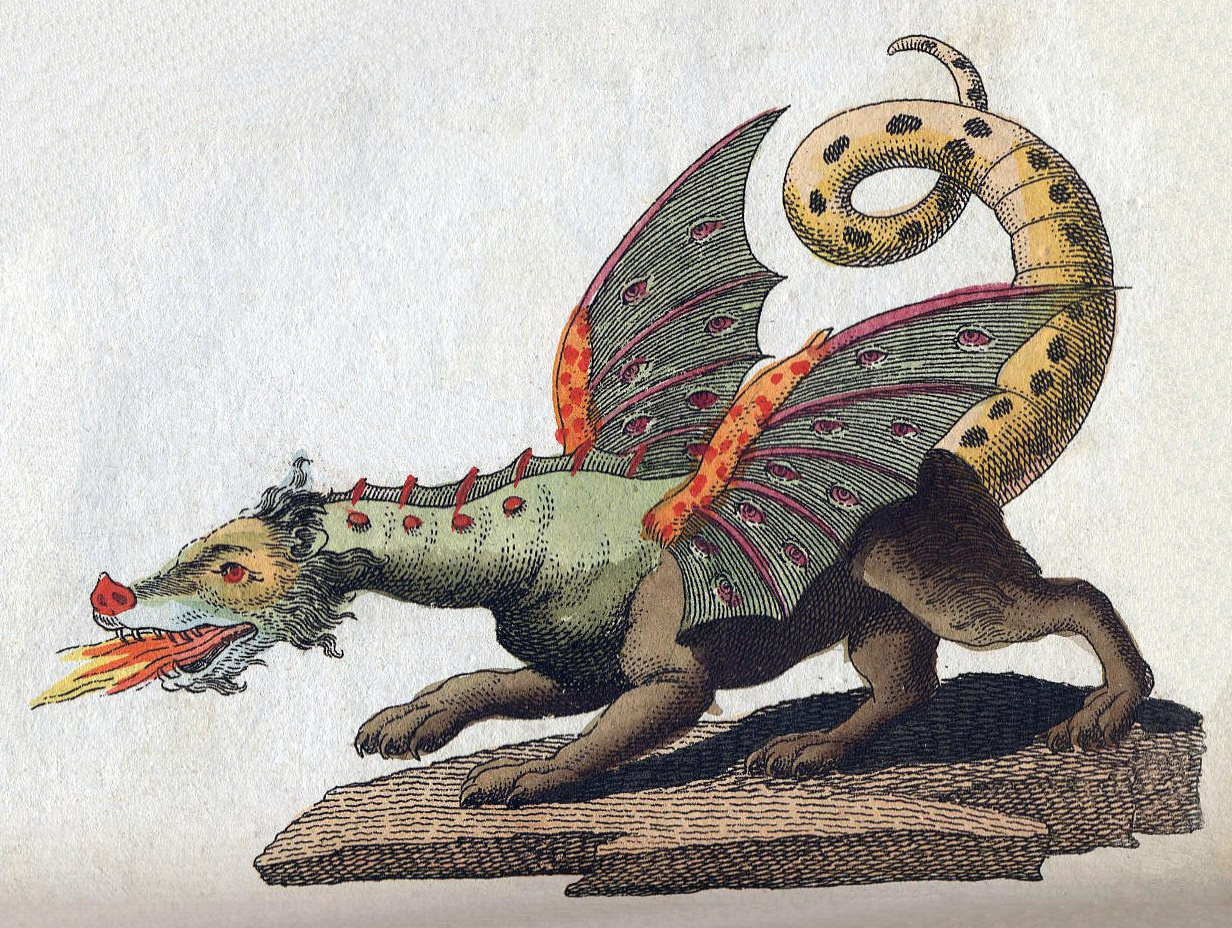
\includegraphics{images/Dragon1.jpeg} Medieval
Dragon(\href{https://en.wikipedia.org/wiki/Dragon}{Source}))

Cartoon Dragon 
\includegraphics{images/Dragon2.jpeg}\\
Cartoon Dragon
(\href{https://www.istockphoto.com/vector/cartoon-dragon-posing-with-fire-gm486859494-73500809}{Source}))

Flying Dragon 
\includegraphics{images/Dragon3.png} Flying Dragon
(\href{https://www.feedyourdragon.com/about.html}{Source}))

\begin{Shaded}
\begin{Highlighting}[]
\FunctionTok{library}\NormalTok{(ggplot2)}
\FunctionTok{library}\NormalTok{(ape)}
\FunctionTok{library}\NormalTok{(knitr)}
\FunctionTok{library}\NormalTok{(reshape2)}
\FunctionTok{library}\NormalTok{(ggtree)}
\end{Highlighting}
\end{Shaded}

\begin{verbatim}
## ggtree v3.2.1  For help: https://yulab-smu.top/treedata-book/
## 
## If you use ggtree in published research, please cite the most appropriate paper(s):
## 
## 1. Guangchuang Yu. Using ggtree to visualize data on tree-like structures. Current Protocols in Bioinformatics. 2020, 69:e96. doi:10.1002/cpbi.96
## 2. Guangchuang Yu, Tommy Tsan-Yuk Lam, Huachen Zhu, Yi Guan. Two methods for mapping and visualizing associated data on phylogeny using ggtree. Molecular Biology and Evolution. 2018, 35(12):3041-3043. doi:10.1093/molbev/msy194
## 3. Guangchuang Yu, David Smith, Huachen Zhu, Yi Guan, Tommy Tsan-Yuk Lam. ggtree: an R package for visualization and annotation of phylogenetic trees with their covariates and other associated data. Methods in Ecology and Evolution. 2017, 8(1):28-36. doi:10.1111/2041-210X.12628
\end{verbatim}

\begin{verbatim}
## 
## Attaching package: 'ggtree'
\end{verbatim}

\begin{verbatim}
## The following object is masked from 'package:ape':
## 
##     rotate
\end{verbatim}

\begin{Shaded}
\begin{Highlighting}[]
\FunctionTok{library}\NormalTok{(ggimage)}
\end{Highlighting}
\end{Shaded}

\begin{Shaded}
\begin{Highlighting}[]
\CommentTok{\# Importing Data}
\NormalTok{DragonNexus }\OtherTok{\textless{}{-}} \FunctionTok{read.nexus.data}\NormalTok{(}\StringTok{"input/DragonMatrix.nex"}\NormalTok{)}
\NormalTok{WeightsDat }\OtherTok{\textless{}{-}} \FunctionTok{read.csv}\NormalTok{(}\StringTok{"https://colauttilab.github.io/Data/Weights.csv"}\NormalTok{)}
\end{Highlighting}
\end{Shaded}

\begin{Shaded}
\begin{Highlighting}[]
\CommentTok{\# Creating a single vector of weights}
\NormalTok{Weights }\OtherTok{\textless{}{-}} \FunctionTok{paste0}\NormalTok{(WeightsDat}\SpecialCharTok{$}\NormalTok{Weight,}\AttributeTok{collapse=}\StringTok{""}\NormalTok{)}
\NormalTok{Weights }\OtherTok{\textless{}{-}} \FunctionTok{strsplit}\NormalTok{(Weights,}\AttributeTok{split=}\StringTok{""}\NormalTok{)[[}\DecValTok{1}\NormalTok{]]}

\CommentTok{\# Converting each letter to a value}
\NormalTok{WeightsNum }\OtherTok{\textless{}{-}} \FunctionTok{rep}\NormalTok{(}\ConstantTok{NA}\NormalTok{,}\FunctionTok{length}\NormalTok{(Weights))}
\ControlFlowTok{for}\NormalTok{(i }\ControlFlowTok{in} \DecValTok{1}\SpecialCharTok{:}\FunctionTok{length}\NormalTok{(WeightsNum))\{}
  \ControlFlowTok{if}\NormalTok{(Weights[i] }\SpecialCharTok{\%in\%}\NormalTok{ LETTERS)\{}
\NormalTok{    WeightsNum[i] }\OtherTok{\textless{}{-}} \FunctionTok{which}\NormalTok{(LETTERS }\SpecialCharTok{==}\NormalTok{ Weights[i]) }\SpecialCharTok{+} \DecValTok{9}
\NormalTok{  \} }\ControlFlowTok{else}\NormalTok{ \{}
\NormalTok{    WeightsNum[i] }\OtherTok{\textless{}{-}}\NormalTok{ Weights[i]}
\NormalTok{  \}}
\NormalTok{\}}
\CommentTok{\# Creating list of weights}
\NormalTok{WeightsNum }\OtherTok{\textless{}{-}} \FunctionTok{as.numeric}\NormalTok{(WeightsNum)}

\CommentTok{\# Multiplying the weight value by the trait vector for each dragon.}
\NormalTok{WtDragonNexus }\OtherTok{\textless{}{-}}\NormalTok{ DragonNexus}
\ControlFlowTok{for}\NormalTok{ (i }\ControlFlowTok{in} \DecValTok{1}\SpecialCharTok{:}\FunctionTok{length}\NormalTok{(DragonNexus))\{}
\NormalTok{  RepWeight }\OtherTok{\textless{}{-}}\NormalTok{ DragonNexus[[i]] }\SpecialCharTok{==} \DecValTok{1}
\NormalTok{  WtDragonNexus[[i]][RepWeight] }\OtherTok{\textless{}{-}}\NormalTok{ WeightsNum[RepWeight]}
\NormalTok{  RepWeight }\OtherTok{\textless{}{-}} \ConstantTok{NA}
\NormalTok{\}}

\NormalTok{WtDragonNexusDF }\OtherTok{\textless{}{-}} \FunctionTok{data.frame}\NormalTok{(}\FunctionTok{matrix}\NormalTok{(}\FunctionTok{unlist}\NormalTok{(WtDragonNexus), }\AttributeTok{ncol=}\FunctionTok{length}\NormalTok{(DragonNexus[[}\DecValTok{1}\NormalTok{]]), }\AttributeTok{byrow=}\NormalTok{T))}
\FunctionTok{row.names}\NormalTok{(WtDragonNexusDF) }\OtherTok{\textless{}{-}} \FunctionTok{names}\NormalTok{(WtDragonNexus)}
\NormalTok{WtDragonDist }\OtherTok{\textless{}{-}} \FunctionTok{dist}\NormalTok{(WtDragonNexusDF,}\AttributeTok{method=}\StringTok{\textquotesingle{}euclidean\textquotesingle{}}\NormalTok{)}
\end{Highlighting}
\end{Shaded}

\begin{verbatim}
## Warning in dist(WtDragonNexusDF, method = "euclidean"): NAs introduced by
## coercion
\end{verbatim}

\begin{Shaded}
\begin{Highlighting}[]
\CommentTok{\# Plotting the Phylogeny}
\NormalTok{WtDragonTree }\OtherTok{\textless{}{-}} \FunctionTok{fastme.bal}\NormalTok{(WtDragonDist)}
\CommentTok{\# Removing X\textquotesingle{}s from the labels}
\NormalTok{WtDragonTree}\SpecialCharTok{$}\NormalTok{tip.label }\OtherTok{\textless{}{-}} \FunctionTok{gsub}\NormalTok{(}\StringTok{"([\^{}X]+)X*"}\NormalTok{, }\StringTok{"}\SpecialCharTok{\textbackslash{}\textbackslash{}}\StringTok{1"}\NormalTok{, WtDragonTree}\SpecialCharTok{$}\NormalTok{tip.label)  }
\CommentTok{\# Colouring the new species added a different colour}
\NormalTok{WtDragonTree }\OtherTok{\textless{}{-}} \FunctionTok{groupClade}\NormalTok{(WtDragonTree, }\AttributeTok{.node =} \FunctionTok{c}\NormalTok{(}\DecValTok{122}\NormalTok{, }\DecValTok{123}\NormalTok{))  }
\FunctionTok{ggtree}\NormalTok{(WtDragonTree, }\AttributeTok{layout =} \StringTok{\textquotesingle{}fan\textquotesingle{}}\NormalTok{, }\AttributeTok{branch.length =} \StringTok{\textquotesingle{}none\textquotesingle{}}\NormalTok{, }\FunctionTok{aes}\NormalTok{(}\AttributeTok{colour =}\NormalTok{ group)) }\SpecialCharTok{+} \FunctionTok{geom\_tiplab}\NormalTok{(}\AttributeTok{size =} \DecValTok{2}\NormalTok{, }\AttributeTok{hjust =} \SpecialCharTok{{-}}\NormalTok{.}\DecValTok{1}\NormalTok{)  }
\end{Highlighting}
\end{Shaded}

\begin{verbatim}
## Scale for 'y' is already present. Adding another scale for 'y', which will
## replace the existing scale.
\end{verbatim}

\includegraphics{A7_Holmes_Brooke_files/figure-latex/unnamed-chunk-4-1.pdf}
\#\#\# \textbf{Figure 1.}\emph{Phylogenic Tree Plot} \#\#\#\#\# The blue
and green lines represent the dragons I added (Medieval, Cartoon and
Flying). Cartoon and Flying are more related to eachoher than either
with Medieval, although they are closely related to Medieval. They are
most closely related to Japanese dragons.

\end{document}
